%%%%%%%%%%%%%%%%%%%%%%%%%%%%%%%%%%%%%%%%%
% Beamer Presentation
% LaTeX Template
% Version 1.0 (10/11/12)
%
% This template has been downloaded from:
% http://www.LaTeXTemplates.com
%
% License:
% CC BY-NC-SA 3.0 (http://creativecommons.org/licenses/by-nc-sa/3.0/)
%
%%%%%%%%%%%%%%%%%%%%%%%%%%%%%%%%%%%%%%%%%

%----------------------------------------------------------------------------------------
%	PACKAGES AND THEMES
%----------------------------------------------------------------------------------------

\documentclass{beamer}

\mode<presentation> {

% The Beamer class comes with a number of default slide themes
% which change the colors and layouts of slides. Below this is a list
% of all the themes, uncomment each in turn to see what they look like.

%\usetheme{default}
%\usetheme{AnnArbor}
%\usetheme{Antibes}
%\usetheme{Bergen}
%\usetheme{Berkeley}
%\usetheme{Berlin}
%\usetheme{Boadilla}
%\usetheme{CambridgeUS}
%\usetheme{Copenhagen} --
%\usetheme{Darmstadt} --
%\usetheme{Dresden}
%\usetheme{Frankfurt} --
%\usetheme{Goettingen}
%\usetheme{Hannover}
%\usetheme{Ilmenau}
%\usetheme{JuanLesPins}
%\usetheme{Luebeck}
\usetheme{Madrid}
%\usetheme{Malmoe}
%\usetheme{Marburg}
%\usetheme{Montpellier}
%\usetheme{PaloAlto}
%\usetheme{Pittsburgh}
%\usetheme{Rochester}
%\usetheme{Singapore}
%\usetheme{Szeged}
%\usetheme{Warsaw}

% As well as themes, the Beamer class has a number of color themes
% for any slide theme. Uncomment each of these in turn to see how it
% changes the colors of your current slide theme.

%\usecolortheme{albatross}
%\usecolortheme{beaver}
%\usecolortheme{beetle}
%\usecolortheme{crane}
%\usecolortheme{dolphin}
%\usecolortheme{dove}
%\usecolortheme{fly}
%\usecolortheme{lily}
%\usecolortheme{orchid}
%\usecolortheme{rose}
%\usecolortheme{seagull}
%\usecolortheme{seahorse}
%\usecolortheme{whale}
%\usecolortheme{wolverine}

%\setbeamertemplate{footline} % To remove the footer line in all slides uncomment this line
%\setbeamertemplate{footline}[page number] % To replace the footer line in all slides with a simple slide count uncomment this line

%\setbeamertemplate{navigation symbols}{} % To remove the navigation symbols from the bottom of all slides uncomment this line
}

\usepackage[spanish]{babel}
\usepackage[utf8]{inputenc}

\usepackage{graphicx} % Allows including images
\usepackage{booktabs} % Allows the use of \toprule, \midrule and \bottomrule in tables

\usepackage{subcaption}
\captionsetup{compatibility=false}

\renewcommand\footnotemark{}
\renewcommand\footnoterule{}

\usepackage[export]{adjustbox}
\usepackage{wrapfig}

\usepackage{textpos}
\usepackage{color}


\newenvironment{figure*}%
{\begin{figure}}
{\end{figure}}

%----------------------------------------------------------------------------------------
%	TITLE PAGE
%----------------------------------------------------------------------------------------

\title[RRAP]{Proyecto de grado: Routers Reconfigurables de Altas Prestaciones} % The short title appears at the bottom of every slide, the full title is only on the title page

\author{Rodrigo Amaro, Emiliano Viotti}
\institute[UdelaR] % Your institution as it will appear on the bottom of every slide, may be shorthand to save space
{
Instituto de Computaci\'on \\ Facultad de Ingeniería \\ Universidad de la República \\ \vspace{0.2cm} Tutores: Dr. Eduardo Gramp\'in, MSc. Mart\'in Giachino % Your institution for the title page
%\medskip
%\textit{john@smith.com} % Your email address
}
\date{\today} % Date, can be changed to a custom date

\begin{document}

\begin{frame}
\titlepage % Print the title page as the first slide
\end{frame}


\begin{frame}
\frametitle{Agenda} % Table of contents slide, comment this block out to remove it
\tableofcontents % Throughout your presentation, if you choose to use \section{} and \subsection{} commands, these will automatically be printed on this slide as an overview of your presentation
\end{frame}

\definecolor{blue(ryb)}{rgb}{0.01, 0.28, 1.0}

%----------------------------------------------------------------------------------------
%	PRESENTATION SLIDES
%----------------------------------------------------------------------------------------


%------------------------------------------------
\section{Introducci\'on} 
\frame{\tableofcontents[currentsection]}

\begin{frame}
\frametitle{Motivaci\'on I} 

\begin{block}{Redes acad\'emicas}
Internet no parece apropiada para su utilizaci\'on en el contexto académico en el desarrollo de nuevos protocolos y servicios, enseñanza, investigaci\'on y la innovaci\'on en el \'area.
\end{block}

\begin{figure}[h] 
\centering    
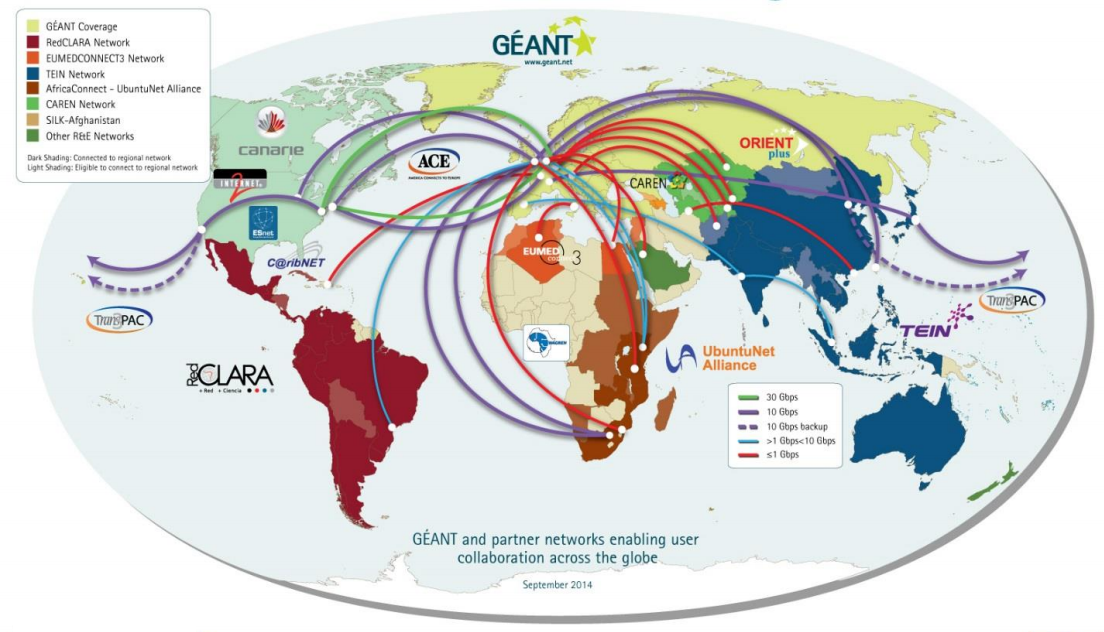
\includegraphics[width=0.7\textwidth]{imagenes/redesAcademicas.png}
\label{fig:AcademicNetworks}
\end{figure}

\end{frame}

\begin{frame}
\frametitle{Motivaci\'on II} 

\begin{block}{Red Académica Uruguaya (RAU)}
A nivel local, la RAU es un emprendimiento de la Universidad de la República administrado por el SeCIU con los objetivos de unir a las instituciones académicas nacionales en una red de alcance nacional y a trav\'es de ella conectarlas a Latinoam\'erica. 
\end{block}

\begin{block}{RAU2}
Remplazo de la actual red académica, es una red avanzada de altas prestaciones que estar\'ia dotada de funciones de virtualizaci\'on de redes flexibles en su definici\'on y uso.
\end{block}

\begin{figure}[h] 
\centering    

\includegraphics[width=0.3\textwidth]{imagenes/logorau2.png}
\label{fig:RAU}
\end{figure}

\end{frame}

\begin{frame}
\frametitle{Motivaci\'on III} 

\begin{block}{Hardware comercial}
Los equipos de red de backbone comerciales como HP, CISCO, Juniper son costos y generalmente de naturaleza cerrada. Las funcionalidades del hardware se restringen a las funcionalidades expuesta por
una API propietaria. 
\end{block}

\begin{figure}[htp]
\centering
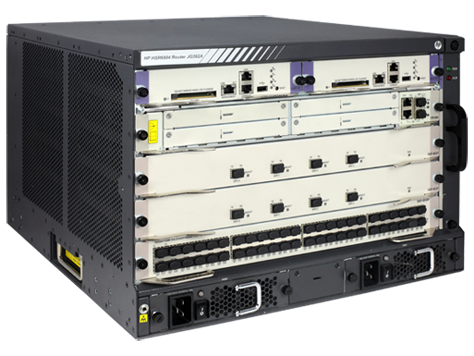
\includegraphics[width=.25\textwidth]{imagenes/corerouter2.png}\hfill
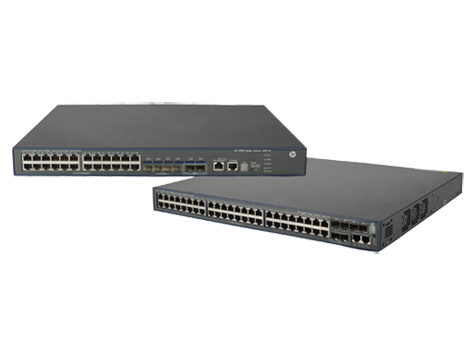
\includegraphics[width=.35\textwidth]{imagenes/corerouter1.png}\hfill
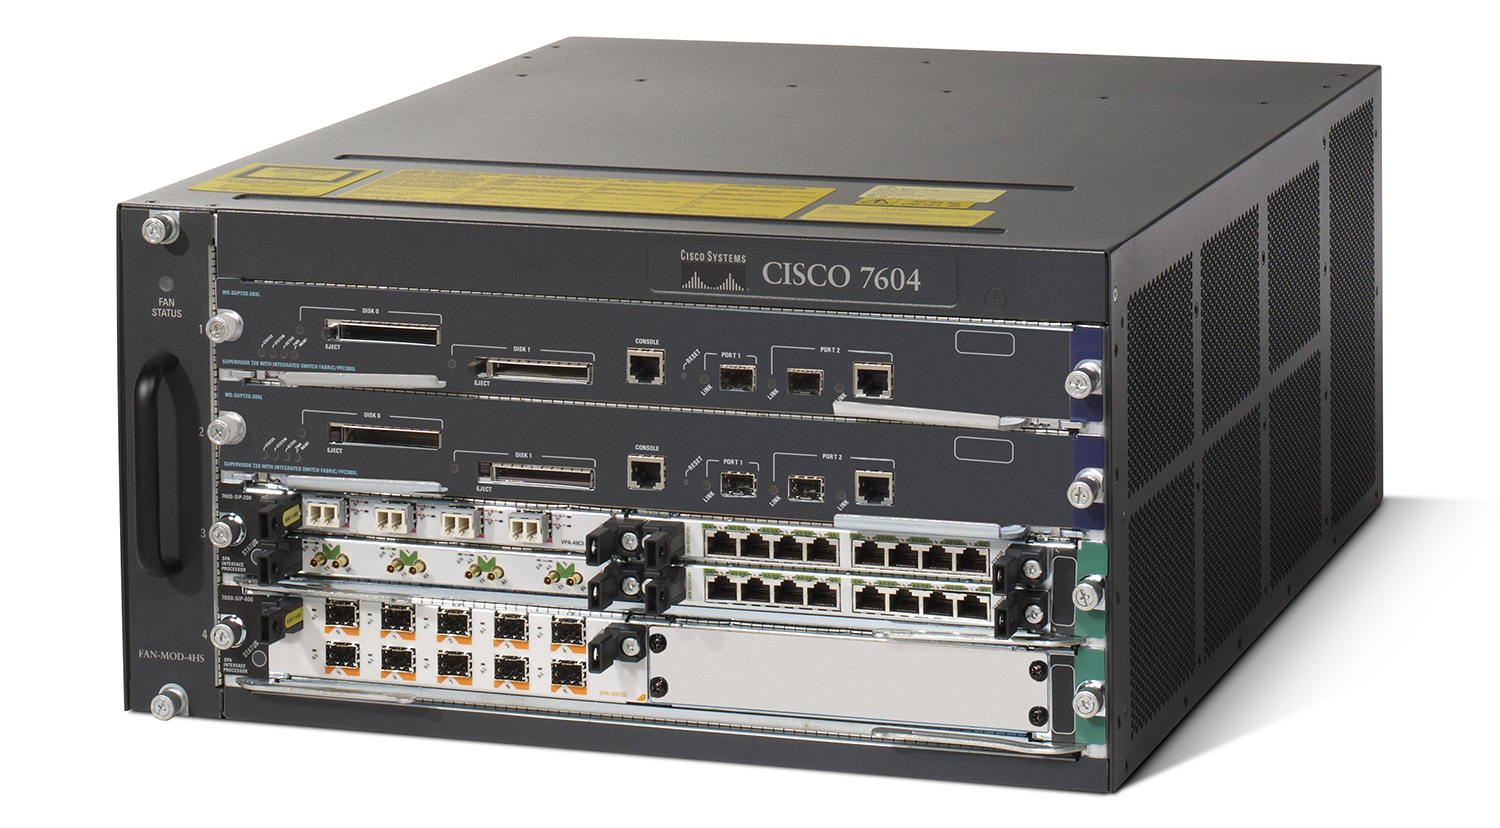
\includegraphics[width=.35\textwidth]{imagenes/corerouter3.jpg}
\label{fig:figure3}
\end{figure}
\end{frame}

\begin{frame}
\frametitle{Definición del problema I} 

\begin{block}{Definición del Problema }
Constru\'ir un prototipo para la RAU2 utilizando como plataforma PCs con placas de red aceleradas en hardware reconfigurable NetFPGA y el enfoque de las Redes Definidas por Software (SDN).
\end{block}

\pause
\begin{block}{Resultados esperados}
\begin{itemize}
\item Estado del arte en Redes Definidas por Software y hardware NetFPGA
\pause
\item Prototipo de aplicaci\'on de gesti\'on de red utilizando SDN y el hardware NetFPGA enfocado en los requerimientos recabados sobre la RAU2
\pause
\item Diseño e implementaci\'on de pruebas de verificaci\'on para el prototipo construido
\end{itemize}
\end{block}

\end{frame}

\begin{frame}
\frametitle{Definición del problema II} 

Que características se esperan del prototipo, ¿cuales son los requerimientos?

\pause
{\color{blue}R: Veamos cuales son los posibles requerimientos de la RAU2}

\pause
\begin{block}{Requerimientos}
\begin{enumerate}[<+->]
\item Clasificaci\'on y separaci\'on de tr\'afico seg\'un categorías
\item Manejo de grandes vol\'umenes de datos
\item Escalabilidad
\item Red de entrega de contenidos
\end{enumerate}
\end{block}

\pause
Problema demasiado grande!

\end{frame}

%------------------------------------------------

%------------------------------------------------
\section{Conceptos preliminares} 
\frame{\tableofcontents[currentsection]}

\begin{frame}
\frametitle{Enfoque tradicional de redes} 

%SDN presenta un enfoque arquitectonico alternativo al enfoque tradicional de redes.

%Redes definidas %

	\begin{figure}[H]
		\raggedright
		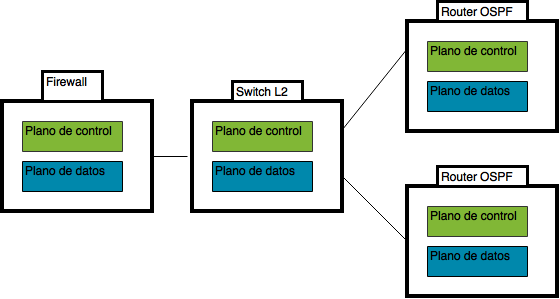
\includegraphics[width=0.5\textwidth, center]{imagenes/SDN-tradicional.png}
	\end{figure}

\hfill

%Enfoque tradicional
%La inteligencia y estado de la red se encuentra distribuida en los mismos dispositivos que reenvian la informacion

\begin{block}{Plano de control}
Es donde reside la inteligencia de la red, es la logica que controla el el comportamiento de reenvio. Ejs : OSPF, RIP,Firewalls
%El cerebro de la red%
\end{block}



\begin{block}{Plano de datos}
Se encarga de reenviar el trafico conforme a el plano de control Ejs : Reenvio IP
 
\end{block}


\end{frame}


\begin{frame}
\frametitle{SDN} 

\begin{block}{Definicion}

La separación física del plano de control de la red del plano de datos, donde el plano
de control controla varios dispositivos.

\end{block}

	\begin{figure}[H]
		\raggedright
		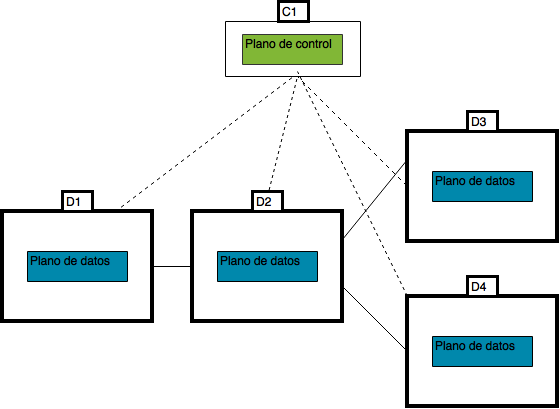
\includegraphics[width=0.5\textwidth, center]{imagenes/SDN-distribuido.png}
	\end{figure}

Escribir algo mas, algun ejemplo. o que ultimamente esta de moda

\end{frame}

\begin{frame}
\frametitle{SDN (Capas l\'ogicas)} 

\begin{itemize}
\item Tres capas: (1) capa de aplicaciones, (2) capa de control y (3) capa de infraestructura
\item Dos interfaces de comunicaci\'on: interfaz sur e interfaz norte
\end{itemize}
 

\begin{figure}[H]
\centering
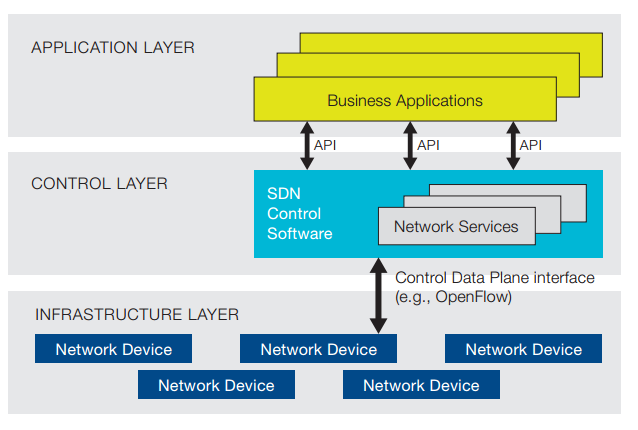
\includegraphics[width=0.6\textwidth]{imagenes/SDNArchitecture.png}
\end{figure}
\end{frame}

\begin{frame}
\frametitle{OpenFlow} 

Soluci\'on basada en el enfoque SDN, ofrece una implementaci\'on est\'andar de la Interfaz Sur (protocolo OpenFlow).


\end{frame}

\begin{frame}
\frametitle{OpenFlow (Capa de Aplicaci\'on)} 

\begin{minipage}{0.40\textwidth}
	\begin{figure}[H]
		\centering
		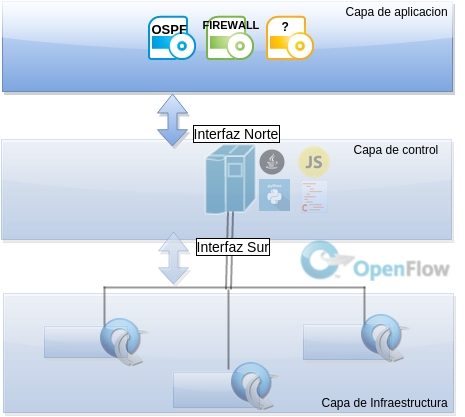
\includegraphics[width=1.0\textwidth]{imagenes/openflowApplication.png}
	\end{figure}

\end{minipage}
\hfill
\begin{minipage}{0.58\textwidth}

Explicar



\end{minipage}

\end{frame}

\begin{frame}
\frametitle{OpenFlow (Capa de Control)} 
\begin{minipage}{0.40\textwidth}
	\begin{figure}[H]
		\centering
		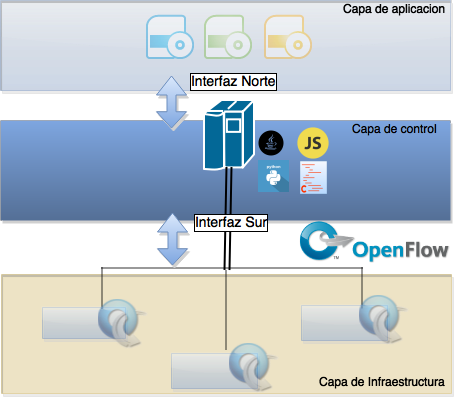
\includegraphics[width=1.0\textwidth]{imagenes/openflowController.png}
	\end{figure}

\end{minipage}
\hfill
\begin{minipage}{0.58\textwidth}
\begin{itemize}
\item Implementaci\'on en Software ejecutada en hardware convencional (x86)
\item Ofrece una API de alto nivel para controlar los dispositivos de una Red (Interfaz Norte)
\item Cada operaci\'on se traduce a reglas OpenFlow e instaladas en el dispositivo a trav\'es de la Interfaz Sur (protocolo OpenFlow)
\end{itemize}

\end{minipage}
\end{frame}

\begin{frame}
\frametitle{OpenFlow (Capa de Dispositivos)} 
\begin{minipage}{0.40\textwidth}
	\begin{figure}[H]
		\centering
		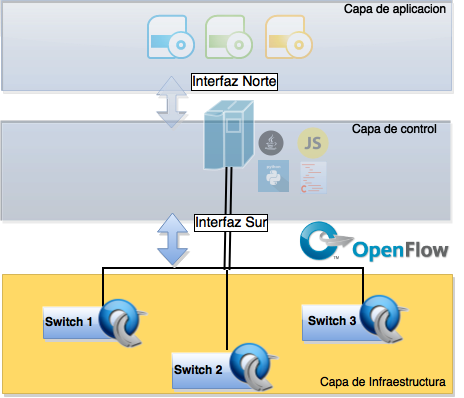
\includegraphics[width=1.0\textwidth]{imagenes/openflowDevices.png}
	\end{figure}

\end{minipage}
\hfill
\begin{minipage}{0.58\textwidth}
Capa de dispositivos
\end{minipage}

\end{frame}

\begin{frame}
\frametitle{VPN (Red privada virtual)} 
Extensión de una red privada sobre la infraestructura de una red pública. Nos interesa diferenciarlas de acuerdo a:
\begin{itemize}
\item Qu\'e capa OSI virtualizan: L2 o L3
\item Conexi\'on utilziada: punto a punto o multipunto
\end{itemize}
	
\vspace{0.4cm}
\begin{figure}[H]
\centering
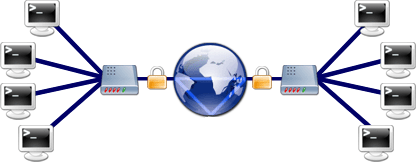
\includegraphics[width=0.65\textwidth]{imagenes/vpn.png}
\end{figure}

\end{frame}

\begin{frame}
\frametitle{MPLS} 

MPLS (Multilabel Protocol Switchig) es la soluci\'on de facto para la implementaci\'on de servicios de VPN L2 y L3. Permite transportar tr\'afico mediante la conmutaci\'on de etiquetas.\\

\vspace{0.4cm}
\pause
Arquitectura:\\

\begin{itemize}
\item Label: Etiqueta MPLS (20bits)
\item Acci\'on: Pop, Push y Swap
\item LSP: Camino de conmutaci\'on de etiquetas
\item FEC: Clase de equivalencia de tr\'afico
\item LDP: Protocolo de distribución de etiquetas
\end{itemize}

\end{frame}


\begin{frame}
\frametitle{NetFPGA} 


	Plataforma de hardware de red reconfigurable y software OpenSource.



%	\begin{block}{Hardware}
		Hardware: Placa PCI-E que cuenta con: 
		\begin{enumerate}
			\item Chip programable FPGA 
			\item 15 GB RAM
			\item 4 Puertos 10-Gigabit Ethernet
		\end{enumerate}
		
	\begin{figure}[H]
		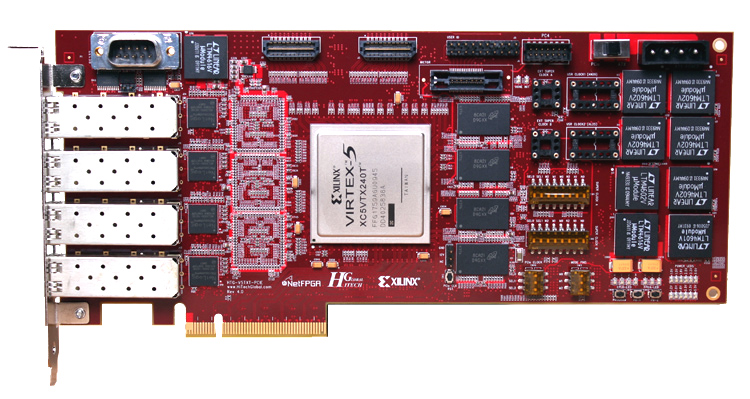
\includegraphics[width=0.65\textwidth, right]{imagenes/NetFPGA10G_web.jpg}
	\end{figure}

%	\end{block}

\end{frame}


\begin{frame}
\frametitle{NetFPGA} 
\begin{block}{Software}
Proyectos de software Open Source que permiten programar comportamientos en el hardware. Dos tipos de proyectos: Referencia y Comunitarios

\end{block}

\begin{table}[]
\small
\centering
\label{label}
\begin{tabular}{| p{3.7cm} | p{6.8cm} |}

\hline
\multicolumn{1}{|l|}{Proyecto \footnote[frame]{\tiny Proyectos NetFPGA extraidos de http://netfpga.org/site/\#/systems/3netfpga-10g/applications/}} & \multicolumn{1}{l|}{Organizaci\'on}\\
\hline
Production Test  & Stanford University \\
Learning CAM Switch &  Stanford University/University of Cambridge \\
Reference NIC 10G  &  Stanford University/University of Cambridge  \\
Reference Router  &  Stanford University/University of Cambridge  \\
\hline
OpenFlow Switch & Stanford University  \\
\hline  
\end{tabular}
\end{table}


\end{frame}






%------------------------------------------------
\section{Arquitectura propuesta} 
\frame{\tableofcontents[currentsection]}

\begin{frame}
\frametitle{Arquitectura propuesta I} 

\begin{itemize}
\item ¿C\'omo implementamos clasificación de tr\'afico y separamos en categorías?

\pause
{\color{blue}R: Construyendo Redes Privadas Virtuales (VPNs)}
\pause

\vspace{0.5cm}
\item ¿C\'omo implementamos Redes Privadas Virtuales?

\pause
{\color{blue}R: Utilizando MPLS (Multilabel Protocol Switch)}

\pause
\vspace{0.5cm}
\item ¿VPNs con MPLS en SDN?

\pause
{\color{blue}R: OpenFlow!}

\end{itemize}

\end{frame}


%\begin{frame}
%\frametitle{Arquitectura propuesta II} 
%
%Utilizamos OpenFlow porque:
%
%\begin{enumerate}[<+->]
%\item Es una implementaci\'on estándar y estable del enfoque SDN
%%Tiene m\'as de 7 a;os en desarrollo, se ha caracterizado por un desarrollo sostenido, ya va por la version 1.5
%\item Adopci\'on de fabricantes de hardware de red
%% Equipos comerciales lo soportan
%\item Gran variedad de software compatible
%\item Esta implementada bajo la filosofía Open Source
%\item OpenFlow incorpora soporte para MPLS desde la versi\'on 1.3.1 del protocolo
%\end{enumerate}
%
%\end{frame}
%

\begin{frame}
\frametitle{Arquitectura propuesta III} 

Se propone una arquitectura h\'ibrida que combina el enfoque SDN con tecnologías actuales, basándose 
en la implementaci\'on de OpenFlow.

\begin{figure}[H]
\centering
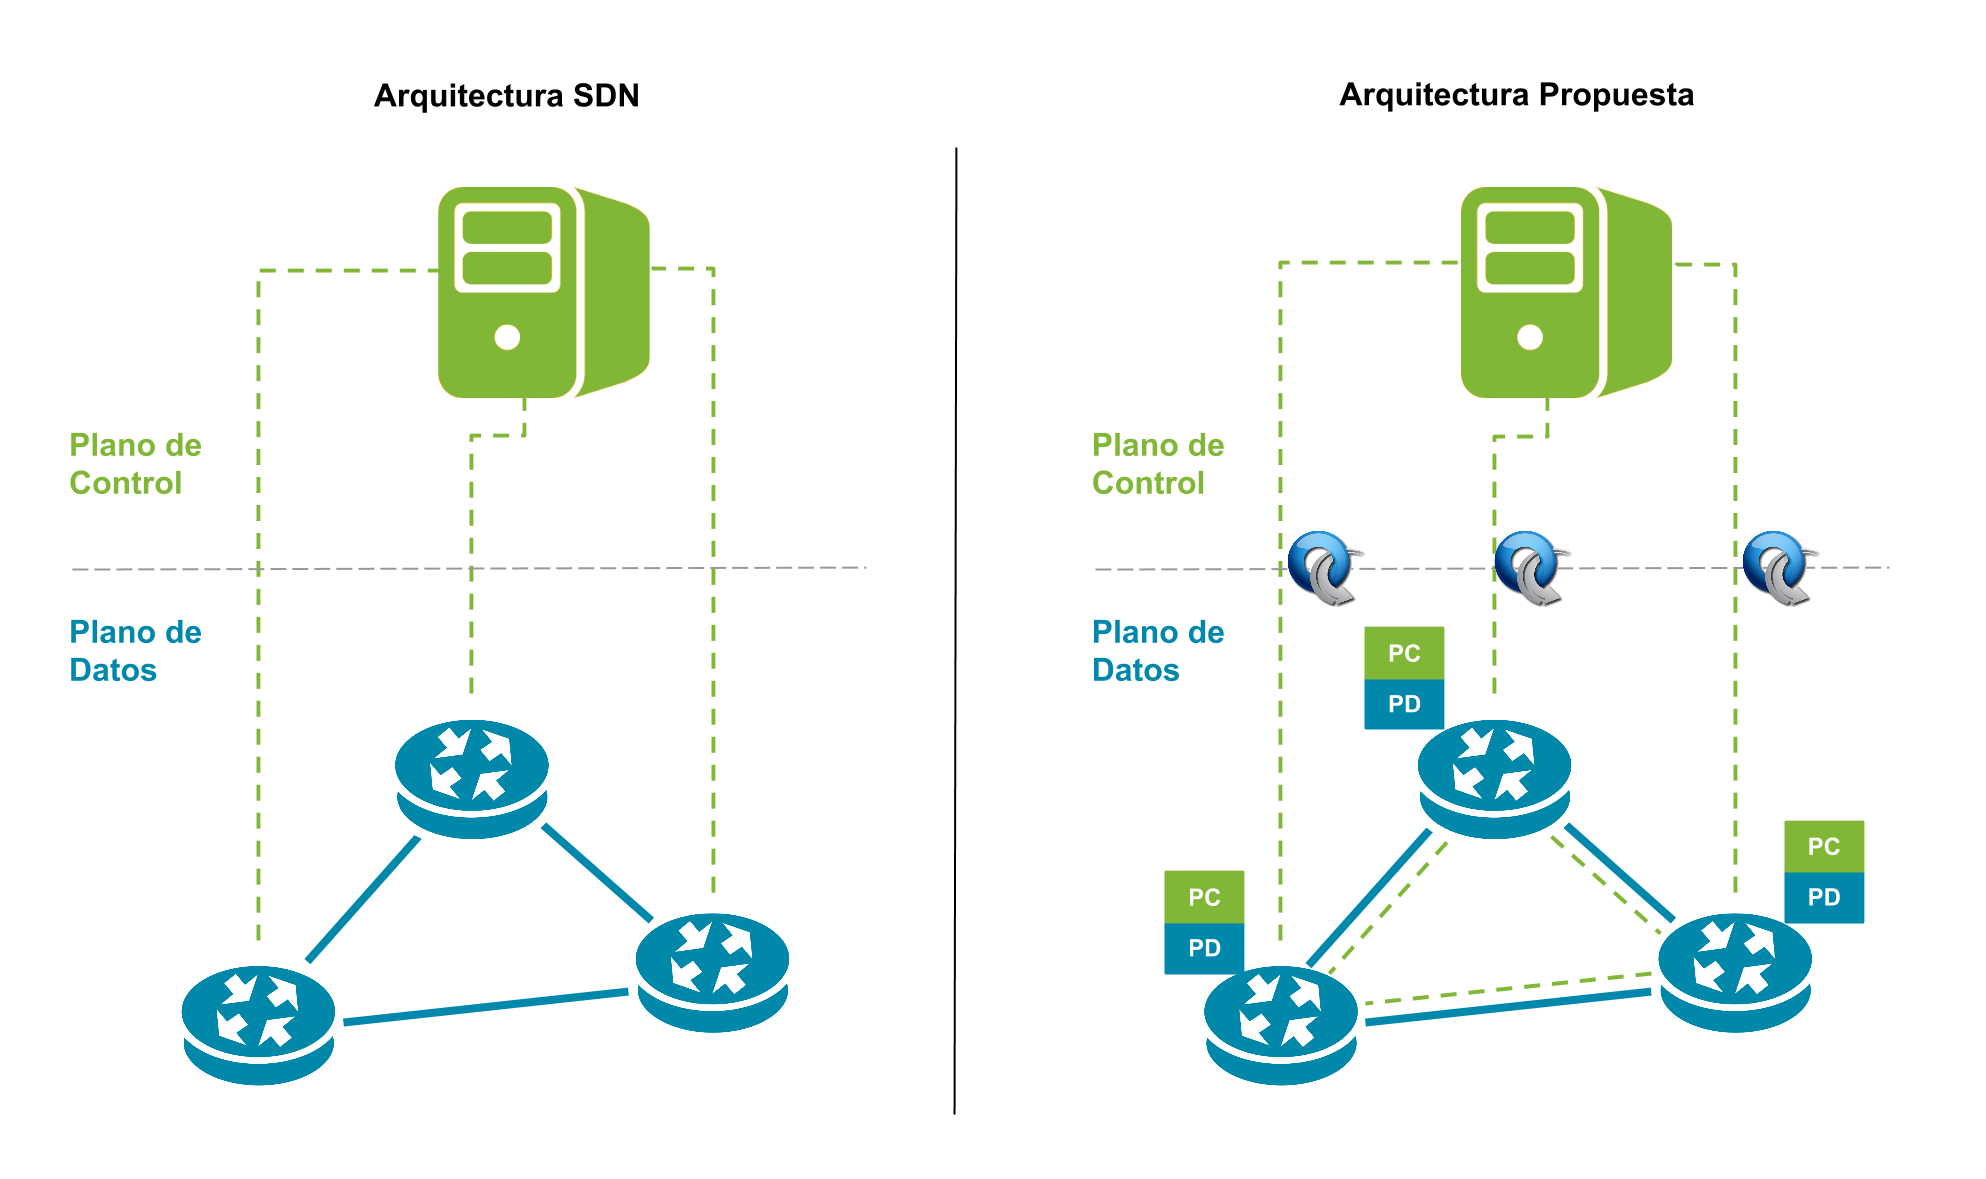
\includegraphics[width=0.95\textwidth, left]{imagenes/arquitecturapropuesta.png}
\end{figure}

\end{frame}


\begin{frame}
\frametitle{Switch OpenFlow} 

Se identifican dos alternativas utilizando hardware NetFPGA:
\pause 
\begin{enumerate}
\item Proyecto OpenFlow
\pause
\item Proyecto ReferenceNIC m\'as implementaci\'on OF en software (Open vSwitch)
\end{enumerate}

\pause
\begin{table}[]
\small
\centering
\label{label}
\begin{tabular}{| p{5cm} | p{5cm} |}

\hline
\multicolumn{1}{|l|}{(1) OpenFlow } & \multicolumn{1}{l|}{(2) ReferenceNIC y OvS } \\
\hline
Velocidad de procesamiento & Prototipaci\'on agil \\
Utilizaci\'on del hardaware &  Tiempo libre para investigaci\'on \\
Conocimiento espec\'ifico &  No hay que utilizar HDLs \\
Licencias full &  Licencias econ\'omicas \\

\hline  
\end{tabular}
\end{table}

\pause
{\color{blue} (2) ReferenceNIC y OvS!}

\end{frame}

\begin{frame}
\frametitle{Controlador OpenFlow} 

Utilizamos Ryu como software de control SDN

\begin{itemize}
\item Compatible con OF hasta v1.4
\item Acad\'emico, sencillo, liviano
\item Libre y Open Source
\end{itemize}

\begin{figure}[H]
\centering
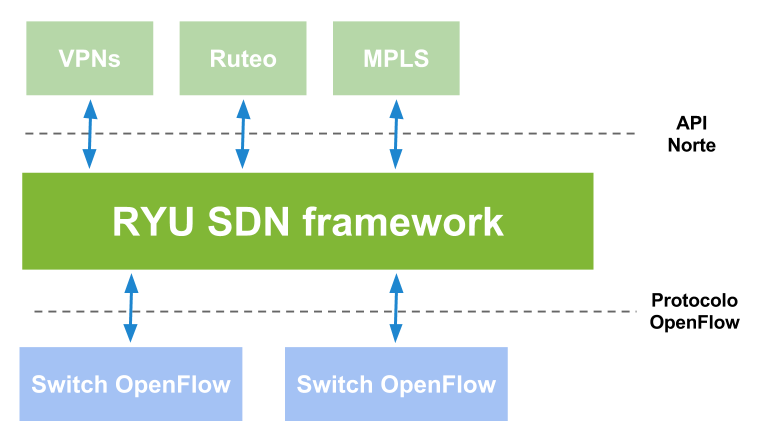
\includegraphics[width=0.65\textwidth]{imagenes/ryuarch.png}
\end{figure}

\end{frame}

\begin{frame}
\frametitle{Algoritmo de Ruteo} 

\begin{itemize}
\item Calculo de rutas en base a IP
\item Utilizamos OSPF para la construcci\'on de una base de datos topol\'ogica (LSDB)
\item Cada nodo en la red incluyendo el controlador ejecutan un demonio OSPF de la herramienta Quagga
\item Algoritmo de ruteo como App SDN en el controlador, toma informaci\'on de la LSDB
\end{itemize}

\end{frame}

\begin{frame}
\frametitle{Agente SNMP} 

\textbf{Agente SNMP} \\
OpenFlow no prev\'e un mecanismo para informar al plano de control direccionamiento IP de un puerto en un dispositivo. \\

\vspace{0.5cm}
\textbf{Soluci\'on:}  Utilizamos un agente SNMP en cada nodo de la red para obtener mapeo entre puertos OF y direcciones IP

\end{frame}

\begin{frame}
\frametitle{Arquitectura Propuesta III} 

\begin{figure}[H]
\centering
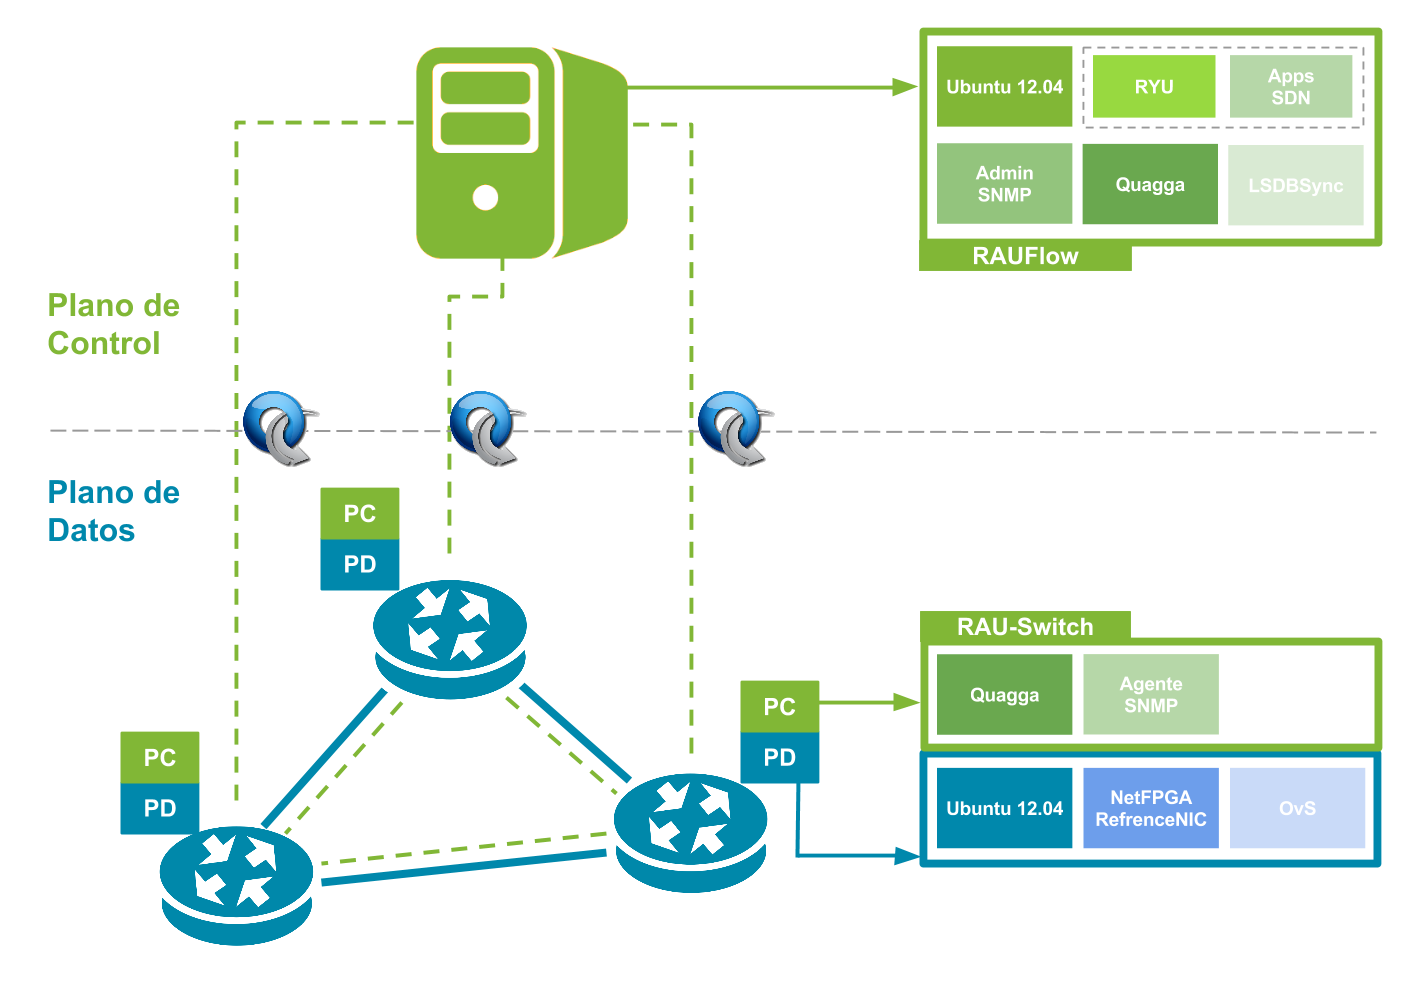
\includegraphics[width=0.80\textwidth]{imagenes/arquitecturapropuesta1.png}
\end{figure}

\end{frame}

%------------------------------------------------

%------------------------------------------------
\section{Implementaci\'on} 
\frame{\tableofcontents[currentsection]}

\begin{frame}
\frametitle{Implementaci\'on I} 

Se implementaron dos componentes:

\begin{enumerate}
\item RAU-Switch: Dispositivo de red compatible con el protocolo OpenFlow
\item RAUFlow: Conjunto de aplicaciones de gesti\'on de redes, implementan plano de control en el prototipo
\end{enumerate}
\end{frame}

\begin{frame}
\frametitle{Implementaci\'on II} 

\begin{figure}[H]
\centering
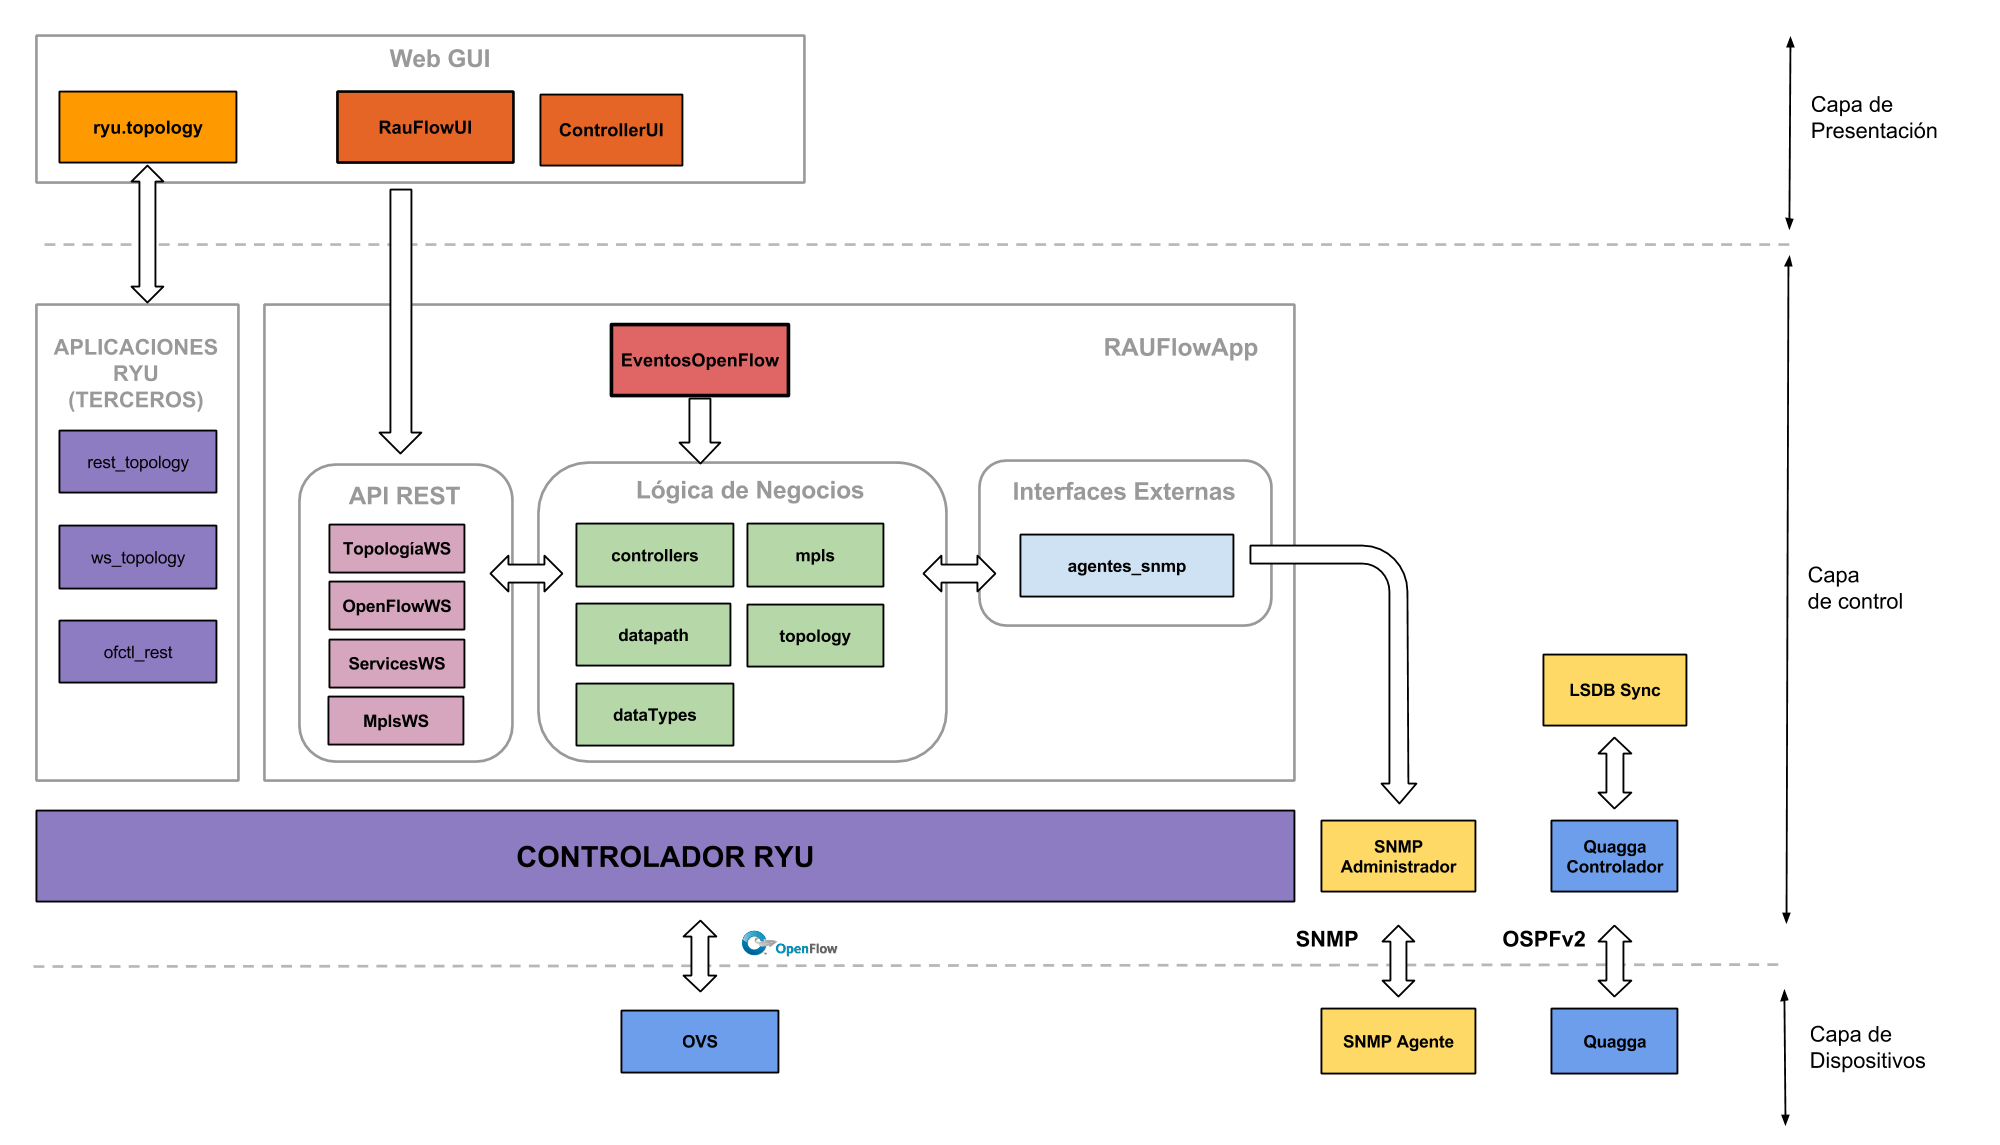
\includegraphics[width=1.0\textwidth]{imagenes/rauflowarquitectura.png}
\end{figure}

\end{frame}
%------------------------------------------------

%------------------------------------------------
\section{Experimentaci\'on} 
\frame{\tableofcontents[currentsection]}

\begin{frame}
\frametitle{Experimentaci\'on} 

Se construye un laboratorio de experimentaci\'on compuesto por 4 nodos RAU-Switch conectados mediante enlaces \'opticos de alta velocidad en una topolog\'ia full Mesh.

\vspace{0.5cm}
\begin{minipage}{0.60\textwidth}
\begin{figure}[htbp]
\centering
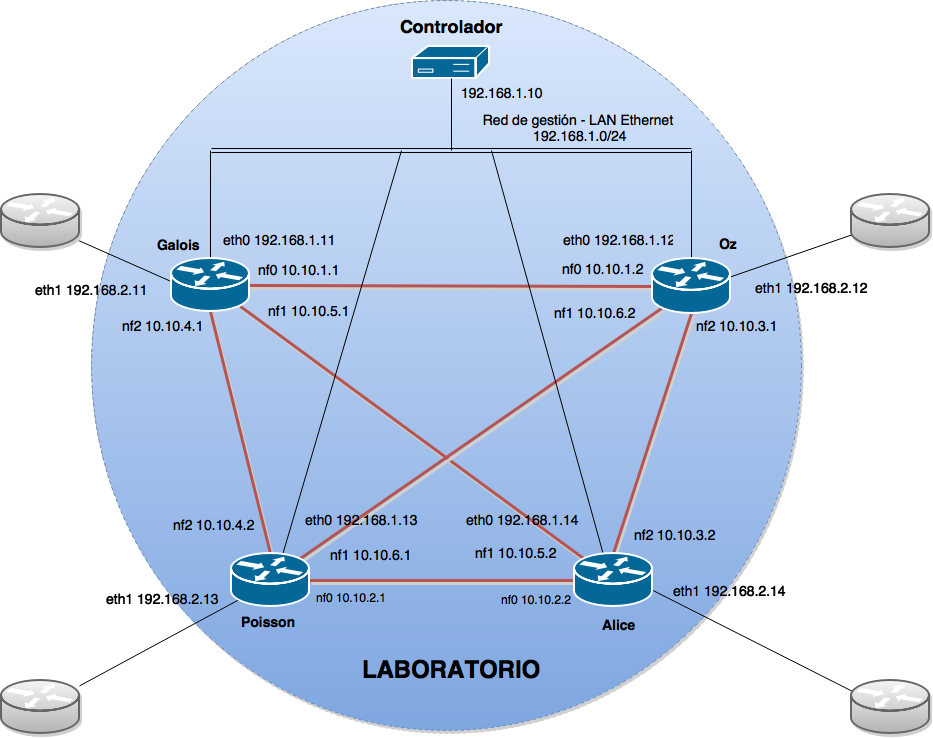
\includegraphics[width=0.81\textwidth]{imagenes/Topologia.png}\hfill
\end{figure}
\end{minipage}
\hfill
\begin{minipage}{0.35\textwidth}
\begin{figure}[H]
\centering
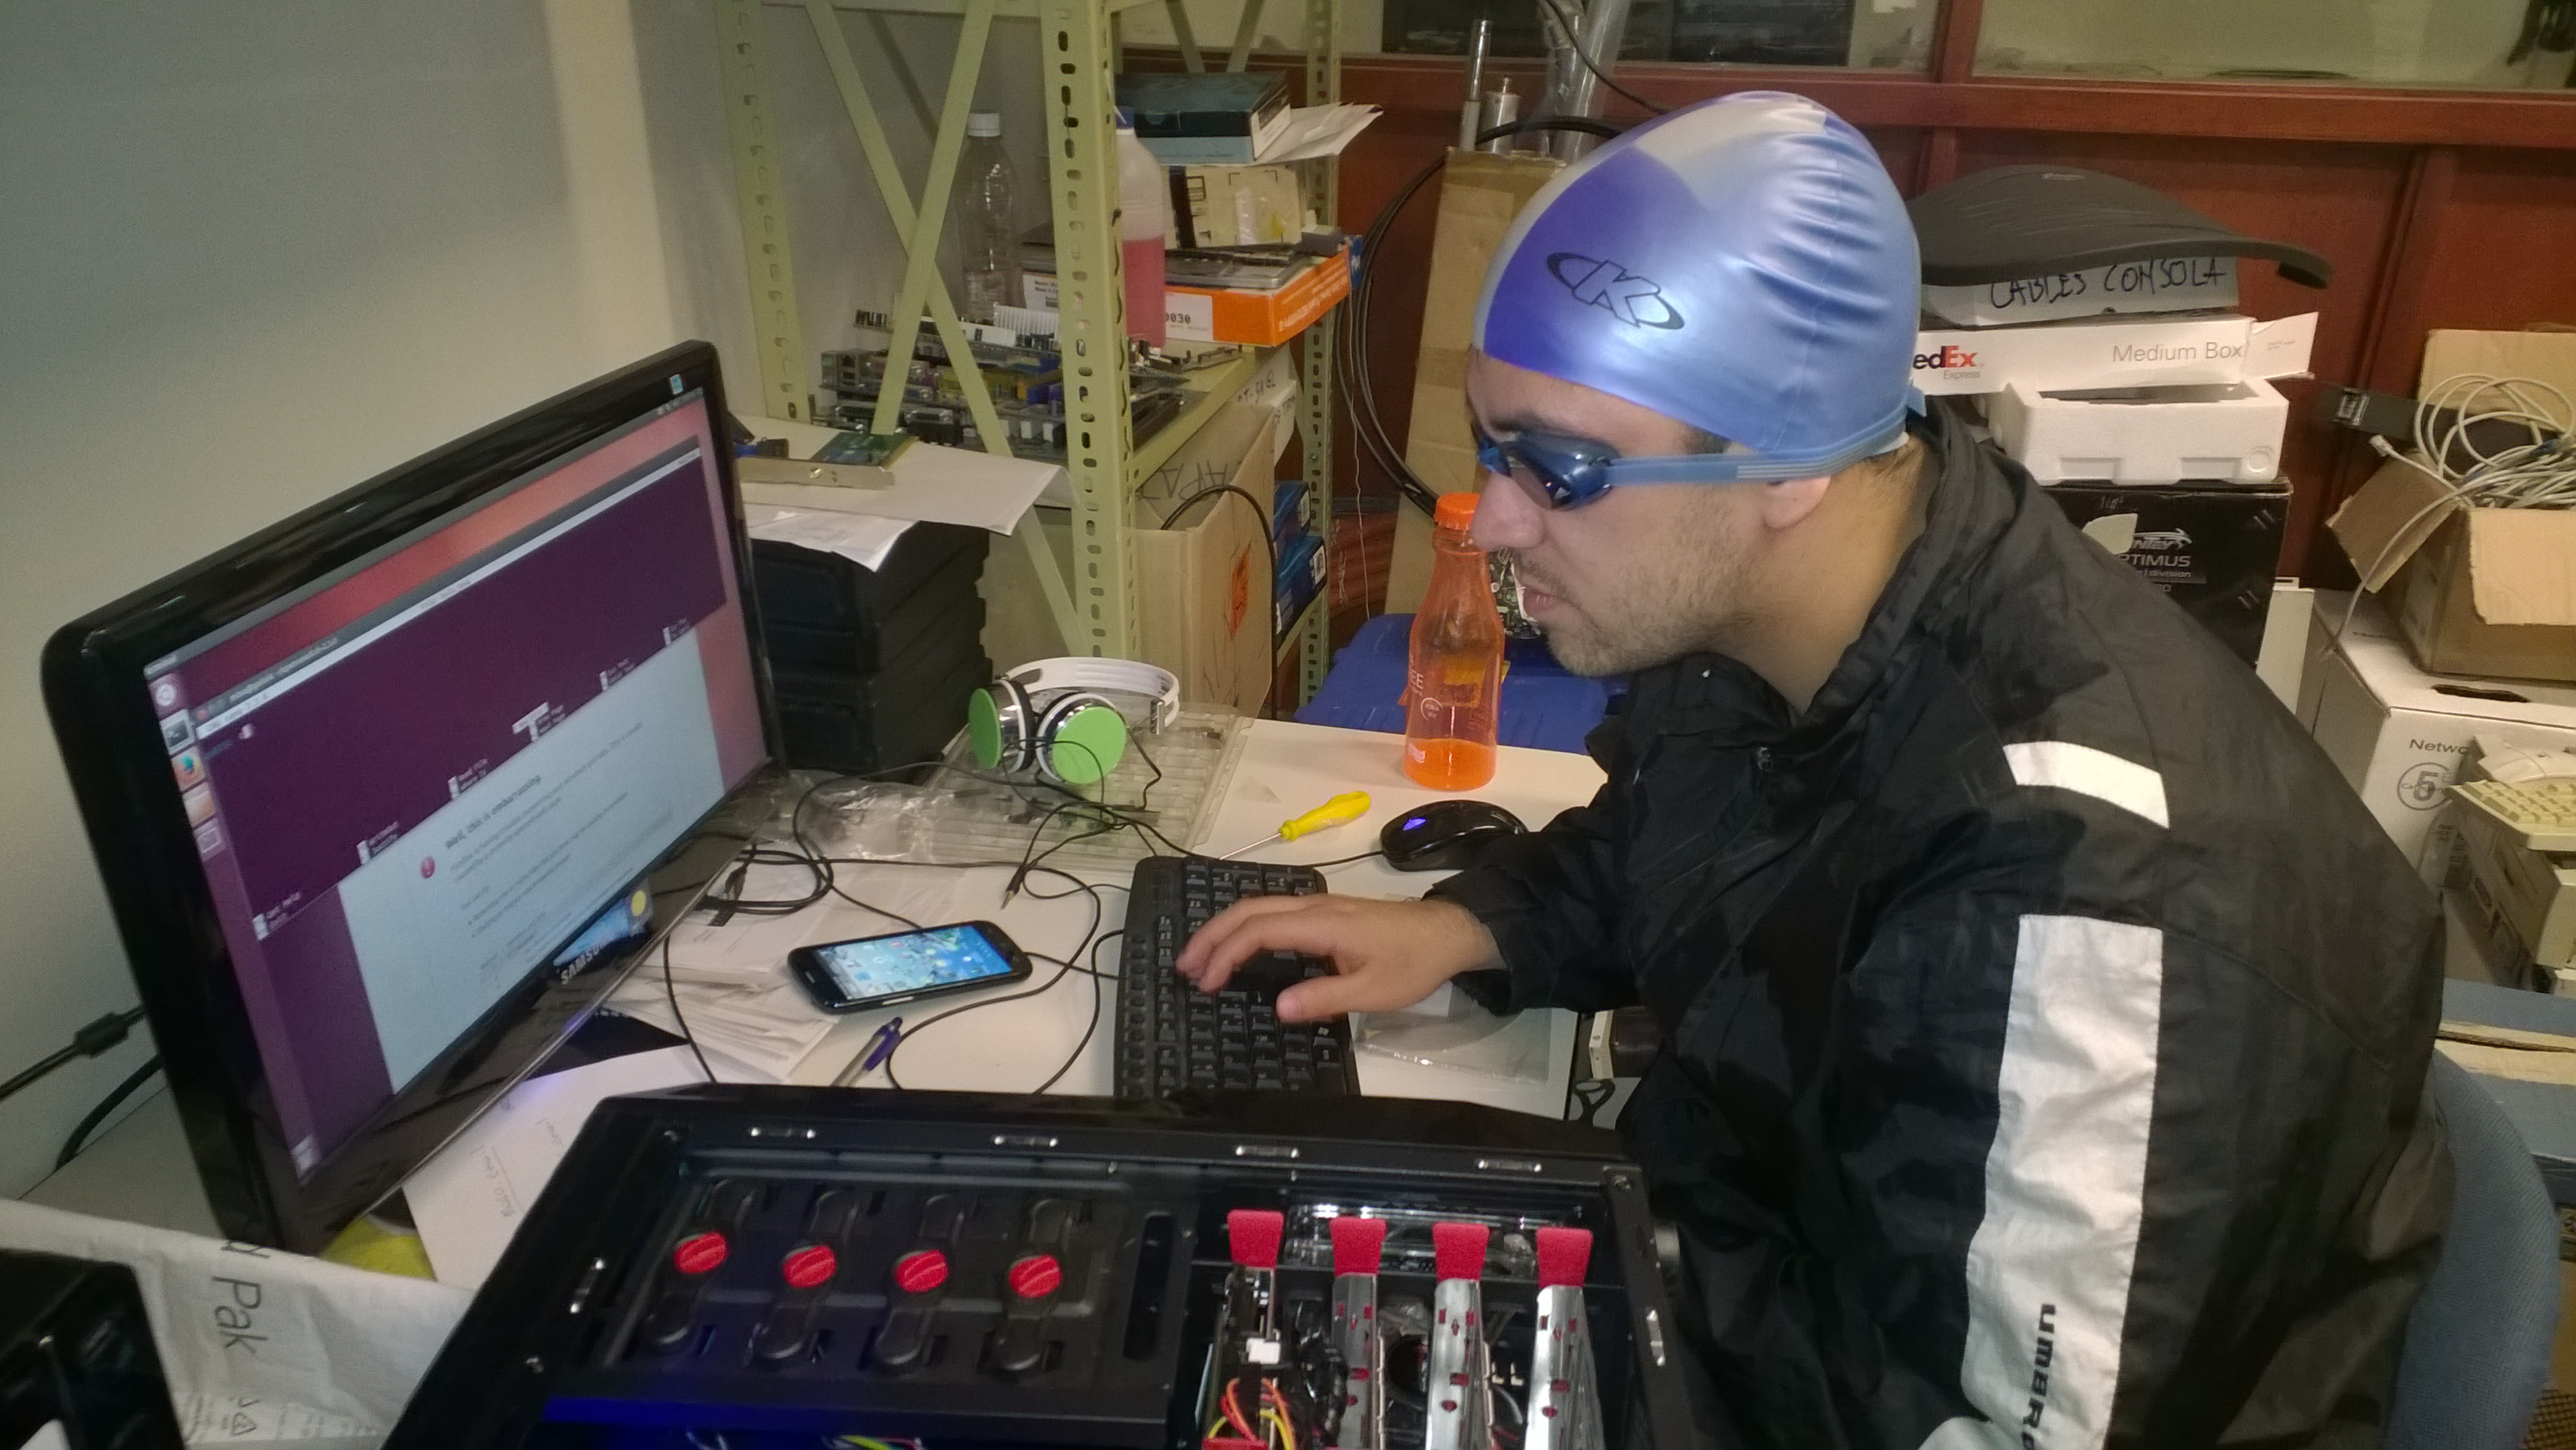
\includegraphics[width=1.0\textwidth]{imagenes/laboratorio.jpg}
\end{figure}
\end{minipage} 

\end{frame}

\begin{frame}
\frametitle{Experimentaci\'on II} 

Mediante la definici\'on de servicios en la aplicaci\'on RAUFlow, se configuran dos tipos de redes privadas:
\begin{enumerate}
\item VPN L3 multipunto
\item VPN L2 punto a punto 
\end{enumerate}


\end{frame}

\begin{frame}
\frametitle{VPN L3} 

Se configuran dos escenarios:

\begin{enumerate}
\item Una organizaci\'on con tres sucursales f\'isicamente separadas
\item Dos organizaciones con dos sucursales f\'isicamente separadas cada una
\end{enumerate}

\vspace{0.4cm}

Las principales características de la implementaci\'on son:
\begin{itemize}
\item Reducci\'on del MTU en 64bits (2 cabezales MPLS)
\item Clasificaci\'on de tr\'afico basada en campos del cabezal OpenFlow
\item Aislamiento del espacio de direcciones IP
\end{itemize}


\end{frame}

\begin{frame}
\frametitle{VPN L2} 

Se configuran un \'unico escenario: Una organizaci\'on con dos sucursales f\'isicamente separadas.

\vspace{0.4cm}

Las principales características de la implementaci\'on son:
\begin{itemize}
\item Reducci\'on del MTU en 64bits (2 cabezales MPLS)
\item Soporte para un conjunto de 43 ethertypes diferentes
\item Se probo diferentes protocolos como ARP, IPv4 IPv6 e IP con tags de VLAN
\end{itemize}


\end{frame}
%------------------------------------------------

%------------------------------------------------
\section{Conclusiones} 
\frame{\tableofcontents[currentsection]}

\begin{frame}
\frametitle{Conclusiones} 

\begin{itemize}
\item Se realiz\'o una investigaci\'on en profundidad del estado del arte de las redes definidas por software (SDN) y la plataforma de hardware NetFPGA.
\end{itemize}
\end{frame}

\begin{frame}
\frametitle{Conclusiones} 

Se implement\'o un prototipo de red de backbone utilizando el hardware NetFPGA y el enfoque SDN:

\pause
\begin{itemize}[<+->]
\item \textbf{RAUswitch} Se construy\'o un router de backbone IP/MPLS compatible con el protocolo OpenFlow y OSPF utilizando el hardware NetFPGA

\item \textbf{RAUflow} Se implement\'o una aplicaci\'on de gesti\'on de red utilizando el enfoque SDN con funcionalidades para la definici\'on de redes privadas virtuales

\begin{itemize}
\item Redefinici\'on del concepto de FEC
\item Clasificaci\'on de tr\'afico mediante protocolo OpenFlow 1.3.1
\item Algoritmo de ruteo din\'amico SPF centralizado
\end{itemize}
\end{itemize}

\end{frame}

\begin{frame}
\frametitle{Conclusiones} 

Se construy\'o un laboratorio de pruebas para la verificaci\'on del prototipo:

\pause
\begin{itemize}[<+->]
\item Se ejecutaron pruebas funcionales

\item Se implementaron dos casos de uso:
\begin{itemize}
\item VPN L3 multipunto
\item VPN L2 punto a punto
\end{itemize}

\end{itemize}

\end{frame}

\begin{frame}
\frametitle{Conclusiones} 

\begin{itemize}[<+->]
\item Se confeccion\'o un manual para la construcci\'on del dispositivo RAUswitch

\item Se contribuy\'o a la comunidad NetFPGA reportando dos BUGs

\item Se escribió un articulo cient\'ifico el cual fue aceptado en la confenrencia Latin American Network Operations and Management Symposium (LANOMS) 2015

\item Se gener\'o un grupo de trabajo (GT SDNUY) uniendo profesionales del SeCIU, Centro de Capacitación y Desarrollo de ANTEL y del Centro Universitario de la Región Este (CURE) 

\end{itemize}

\end{frame}

%Se implement ́o un prototipo de red de backbone utilizando el
%hardware NetFPGA y el enfoque SDN
%Se implement ́o un conjunto de pruebas para la verificaci ́on del
%prototipo construido

%------------------------------------------------

%------------------------------------------------
\section{Trabajo a futuro} 
\frame{\tableofcontents[currentsection]}

\begin{frame}
\frametitle{Trabajo a futuro} 

Se identifican las siguientes l\'ineas de trabajo a futuro:
\pause

\begin{itemize}[<+->]

\item Extender el proyecto OpenFlow de la plataforma NetFPGA para soportar al menos la versi\'on 1.3.1 del protocolo OpenFlow

\item Extender el algoritmo de ruteo SPF para implementar un CSPF

\item Incorporar en RAUFlow la capacidad de soportar m\'ultiples caminos para un mismo Servicio,  balanceo de carga, QoS e Ingenier\'ia de tr\'afico

\end{itemize}

\end{frame}

\begin{frame}
\frametitle{Trabajo a futuro} 

Otras posibles l\'ineas:
\pause
\begin{itemize}[<+->]

\item Agregar una capa de persistencia para ciertos datos

\item Investigar la escalabilidad de RAUflow en topolog\'ias de red realistas 

\item Construir una jerarqu\'ia de controladores e investigar el impacto en el rendimiento 

\item Incorporar m\'as dimensiones a la definici\'on de un servicio (tiempo)

\end{itemize}

\end{frame}

\begin{frame}
\centering
\Huge
¿Preguntas?

\end{frame}

%------------------------------------------------

%----------------------------------------------------------------------------------------

\end{document} 

